
\chapter{SVM gridsearch}\label{apendix:svm_grid}
    All decision boundary plots for the five best and five worst SVM configurations are found below, sorted by score. As can be seen, all five highest scoring configurations produce a very similar decision boundary.  

    \begin{figure}
        \centering
        \includegraphics[width = .7\textwidth]{report/figures/analysis/gridsearch/Novelty detection, 1, training, gamma = 0.05 nu = 1.0583130489998942e-05.png}
        \caption{Decision boundary for OC SVM with parameters $\gamma = 0.05$, $\nu = 1/N$. Score $=0.975$. How to interpret the figure is found in Figure \ref{fig:svm_grid_best}}
        % \label{fig:my_label}
    \end{figure}
    
    \begin{figure}
        \centering
        \includegraphics[width = .7\textwidth]{report/figures/analysis/gridsearch/Novelty detection, 2 training, gamma = 0.1 nu = 5.291565244999471e-05.png}
        \caption{Decision boundary for OC SVM with parameters $\gamma = 0.1$, $\nu = 1/2N$. Score $=0.970$. How to interpret the figure is found in Figure \ref{fig:svm_grid_best}}
        % \label{fig:my_label}
    \end{figure}
    
    \begin{figure}
        \centering
        \includegraphics[width = .7\textwidth]{report/figures/analysis/gridsearch/Novelty detection, 3 training, gamma = 0.1 nu = 0.00010583130489998942.png}
        \caption{Decision boundary for OC SVM with parameters $\gamma = 0.1$, $\nu = 1/N$. Score $=0.961$.How to interpret the figure is found in Figure \ref{fig:svm_grid_best}}
        \label{fig:my_label}
    \end{figure}
    
    \begin{figure}
        \centering
        \includegraphics[width = .7\textwidth]{report/figures/analysis/gridsearch/Novelty detection, 4 training, gamma = 0.05 nu = 0.00021166260979997884.png}
        \caption{Decision boundary for OC SVM with parameters $\gamma = 0.05$, $\nu = 2/N$. Score $=0.960$. How to interpret the figure is found in Figure \ref{fig:svm_grid_best}}
        \label{fig:my_label}
    \end{figure}
    
    \begin{figure}
        \centering
        \includegraphics[width = .7\textwidth]{report/figures/analysis/gridsearch/Novelty detection, 5 training, gamma = 0.2 nu = 0.00010583130489998942.png}
        \caption{Decision boundary for OC SVM with parameters $\gamma = 0.2$, $\nu = 1/N$. Score $=0.957$. How to interpret the figure is found in Figure \ref{fig:svm_grid_best}}
        \label{fig:my_label}
    \end{figure}
    
    
    \begin{figure}
        \centering
        \includegraphics[width = .7\textwidth]{report/figures/analysis/gridsearch/Novelty detection, -5 training, gamma = 8 nu = 1.0583130489998942e-05.png}
        \caption{Decision boundary for OC SVM with parameters $\gamma = 8$, $\nu = 1/10N5$. Score $=-44.437$. How to interpret the figure is found in Figure \ref{fig:svm_grid_best}}
        \label{fig:my_label}
    \end{figure}
    
    \begin{figure}
        \centering
        \includegraphics[width = .7\textwidth]{report/figures/analysis/gridsearch/Novelty detection, -4 training, gamma = 8 nu = 4.233252195999577e-06.png}
        \caption{Decision boundary for OC SVM with parameters $\gamma = 8$, $\nu = 1/25N$. Score $=-51.780$. How to interpret the figure is found in Figure \ref{fig:svm_grid_best}}
        \label{fig:my_label}
    \end{figure}
    
    \begin{figure}
        \centering
        \includegraphics[width = .7\textwidth]{report/figures/analysis/gridsearch/Novelty detection, -3 training, gamma = 0.1 nu = 4.233252195999577e-06.png}
        \caption{Decision boundary for OC SVM with parameters $\gamma = 0.1$, $\nu = 1/25N$. Score $=-57.461$. How to interpret the figure is found in Figure \ref{fig:svm_grid_best}}
        \label{fig:my_label}
    \end{figure}
    
    
    \begin{figure}
        \centering
        \includegraphics[width = .7\textwidth]{report/figures/analysis/gridsearch/Novelty detection, -2 training, gamma = 16 nu = 1.0583130489998942e-05.png}
        \caption{Decision boundary for OC SVM with parameters $\gamma = 16$, $\nu = 1/10N$. Score $=-71.082$. How to interpret the figure is found in Figure \ref{fig:svm_grid_best}}
        \label{fig:my_label}
    \end{figure}
    
    
    \begin{figure}
        \centering
        \includegraphics[width = .7\textwidth]{report/figures/analysis/gridsearch/Novelty detection, -1 training, gamma = 16 nu = 4.233252195999577e-06.png}
        \caption{Decision boundary for OC SVM with parameters $\gamma = 16$, $\nu = 1/25N$. Score $=-506.263$. How to interpret the figure is found in Figure \ref{fig:svm_grid_best}}
        \label{fig:my_label}
    \end{figure}

\chapter{LSTM gridsearch}\label{appendix:lstm_grid}
    The model history for the training of the five best and five worst LSTM configurations are plotted below, from best to worst. As can be seen the worst configurations are stopped after only a few epochs due to lack of improvement of the predictions of the network. 
    \begin{figure}
        \begin{minipage}[b]{0.49\linewidth}
            \centering
            \includegraphics[width = \textwidth]{report/figures/analysis/lstm_gridsearch/best_lstm_error_zoomed.png}
            \caption{Training history for the best LSTM configuration. Test and training prediction error is shown as a function of epochs.}
            % \label{fig:lstm_grid_error_best_appendix}
        \end{minipage}
        \hfill\vline\hfill
        \begin{minipage}[b]{0.49\linewidth}
            \centering
            \includegraphics[width = \textwidth]{report/figures/analysis/lstm_gridsearch/best_lstm_error_2_zoomed.png}
            \caption{Training history for the second best LSTM configuration. Test and training prediction error is shown as a function of epochs.}
            % \label{fig:lstm_grid_error_worst_appendix}
        \end{minipage}
    \end{figure}

    \begin{figure}
        \begin{minipage}[b]{0.49\linewidth}
            \centering
            \includegraphics[width = \textwidth]{report/figures/analysis/lstm_gridsearch/best_lstm_error_3_zoomed.png}
            \caption{Training history for the third best LSTM configuration. Test and training prediction error is shown as a function of epochs.}
            % \label{fig:lstm_grid_error_best_appendix}
        \end{minipage}
        \hfill\vline\hfill
        \begin{minipage}[b]{0.49\linewidth}
            \centering
            \includegraphics[width = \textwidth]{report/figures/analysis/lstm_gridsearch/worst_lstm_error_-3.png}
            \caption{Training history for the fourth best LSTM configuration. Test and training prediction error is shown as a function of epochs.}
            % \label{fig:lstm_grid_error_worst_appendix}
        \end{minipage}
    \end{figure}

    \begin{figure}
        \begin{minipage}[b]{0.49\linewidth}
            \centering
            \includegraphics[width = \textwidth]{report/figures/analysis/lstm_gridsearch/worst_lstm_error_-5.png}
            \caption{Training history for the fifth worst LSTM configuration. Test and training prediction error is shown as a function of epochs.}
            % \label{fig:lstm_grid_error_best_appendix}
        \end{minipage}
        \hfill\vline\hfill
        \begin{minipage}[b]{0.49\linewidth}
            \centering
            \includegraphics[width = \textwidth]{report/figures/analysis/lstm_gridsearch/worst_lstm_error_-4.png}
            \caption{Training history for the fourth worst LSTM configuration. Test and training prediction error is shown as a function of epochs.}
            % \label{fig:lstm_grid_error_worst_appendix}
        \end{minipage}
    \end{figure}

    \begin{figure}
        \begin{minipage}[b]{0.49\linewidth}
            \centering
            \includegraphics[width = \textwidth]{report/figures/analysis/lstm_gridsearch/worst_lstm_error_-3.png}
            \caption{Training history for the third worst LSTM configuration. Test and training prediction error is shown as a function of epochs.}
            % \label{fig:lstm_grid_error_best_appendix}
        \end{minipage}
        \hfill\vline\hfill
        \begin{minipage}[b]{0.49\linewidth}
            \centering
            \includegraphics[width = \textwidth]{report/figures/analysis/lstm_gridsearch/worst_lstm_error_-2.png}
            \caption{Training history for the second worst LSTM configuration. Test and training prediction error is shown as a function of epochs.}
            % \label{fig:lstm_grid_error_worst_appendix}
        \end{minipage}
    \end{figure}
    
    \begin{figure}
        \begin{minipage}[b]{0.45\linewidth}
            \centering
            \includegraphics[width = \textwidth]{report/figures/analysis/lstm_gridsearch/worst_lstm_error_-1.png}
            \caption{Training history for the worst LSTM configuration. Test and training prediction error is shown as a function of epochs.}
            % \label{fig:lstm_grid_error_best_appendix}
        \end{minipage}
    \end{figure}

% \chapter{SVM gridsearch plant 2}
%     A gridsearch after the optimal hyperparameterization for the one class SVM when trained on data from plant 2 is performed. The result is presented in table \ref{tab:svm_gridsearch2}, and the decision boundaries for the two best and two worst parameterizations are seen below. 
%     \begin{table}[h]
%         \centering
%         \begin{tabular}{|c|c|c|}
%             \hline
%              Score  &   $\gamma$    & $\nu$         \\ \hline
%              0.995  &   $0.05$      & $\frac{1}{5N}$ \\ \hline
%              0.987  &   $0.05$      & $\frac{1}{2N}$ \\ \hline
%              0.975  &   $0.05$      & $\frac{1}{N}$ \\ \hline
%              0.972  &   $0.04$      & $\frac{}{10N}$ \\ \hline
%              0.970  &   $0.03$      & $\frac{1}{10N}$ \\ \hline
%              -50.698  &   $10$      & $\frac{1}{10N}$ \\ \hline
%              -91.291  &   $1$      & $\frac{1}{10N}$ \\ \hline
%              -94.296  &   $10$      & $\frac{1}{25N}$ \\ \hline
%              -124.473  &  $0.8$      & $\frac{1}{10N}$ \\ \hline
%              -193.239  &  $5$      & $\frac{1}{25N}$ \\ \hline
             
%         \end{tabular}
%         \caption{Table showing the five best and five worst scores for the gridsearch after optimal hyperparameters for the one class SVM. $N = $ number of samples.}
%         \label{tab:svm_gridsearch2}
%     \end{table}
        
%         \begin{figure}
%             \centering
%             \includegraphics[width = .7\textwidth]{report/figures/analysis/gridsearchPlant2/Novelty detection training, gamma = 0.05 nu = 1.554001554001554e-05.png}
%             \caption{Score = 0.995, #1}
%             \label{fig:my_label}
%         \end{figure}
    
%         \begin{figure}
%             \centering
%             \includegraphics[width = .7\textwidth]{report/figures/analysis/gridsearchPlant2/Novelty detection training, gamma = 0.05 nu = 3.885003885003885e-05.png}
%             \caption{Score = .987, #2}
%             \label{fig:my_label}
%         \end{figure}
        
%         \begin{figure}
%             \centering
%             \includegraphics[width = .7\textwidth]{report/figures/analysis/gridsearchPlant2/Novelty detection training, gamma = 5 nu = 3.108003108003108e-06.png}
%             \caption{Score = -193.239, worst}
%             \label{fig:my_label}
%         \end{figure}
    
%         \begin{figure}
%             \centering
%             \includegraphics[width = .7\textwidth]{report/figures/analysis/gridsearchPlant2/Novelty detection training, gamma = 1 nu = 7.77000777000777e-06.png}
%             \caption{Score = -124.473 second to last wors}
%             \label{fig:my_label}
%         \end{figure}
        
        

\chapter{Training case 1}\label{appendix:training_case1}
    Additional plots from the results of training case 1 is presented below. The plots are discussed in their caption.
    \begin{figure}
        \centering
        \includegraphics[width=0.7\textwidth]{report/figures/analysis/plant1_training/svm_boundary.png}
        \caption{Decision boundary for the OC SVM classifier. Support vectors and training observations are plotted. All samples located outside the red boundary are classified as anomalies. The color indicates the distance to the separating hyperplane.}
        % \label{fig:svm_train_p1_boundary}
    \end{figure}
    
    
     \begin{figure}
        \centering
        \includegraphics[width=0.7\textwidth]{report/figures/analysis/plant1_training/kde_boundary.png}
        \caption{The KDE anomaly scorers probability score plotted as contours in the space of the scaled training data. Training samples are seen in green. As the grid value becomes more and more anomalous the color becomes lighter.}
        \label{fig:my_label}
    \end{figure}
    
    
    \begin{figure}
        \centering
        \includegraphics[width=0.7\textwidth]{report/figures/analysis/plant1_training/lstm_model_error.png}
        \caption{Model error for the LTSM network as the number of epochs increase.}
        % \label{fig:lstm_training_plant1}
    \end{figure}
    
    % \begin{figure}
    %     \centering
    %     \includegraphics[width=\textwidth]{report/figures/analysis/plant1_training/training_data_anomaly.png}
    %     \caption{Anomaly results for the methods trained on training set 1 evaluated on training set 1. How to interpret the figure can be seen in Figure \ref{fig:anomaly_training_set1}. As can be seen the anomaly scores for the KDE and LSTM anomaly scorers are much lower than for case 1 and 2 seen in the results. One datapoint is classified as an outlier by the one class SVM classifier, it is also given a higher anomaly score by the scorers, but is very low compared to the large anomaly scores seen in case 1 and 2.}
    %     % \label{fig:anomaly_training_plant1_case1}
    % \end{figure}
    
    \begin{figure}
        \centering
        \includegraphics[width=\textwidth]{report/figures/analysis/plant1_training/test_data_anomaly.png}
        \caption{Anomaly results for the methods trained on training set 1 evaluated on validation set 1. How to interpret the figure can be seen in Figure \ref{fig:anomaly_training_set1}. As can be seen the anomaly scores for the KDE and LSTM anomaly scorers are much lower than for case 1 and 2 seen in the results, indicating that the scorers correctly evaluates the validation set as normal. The OC SVM classifier correctly classifies all samples as normal.}
        % \label{fig:anomaly_training_plant1}
    \end{figure}

\chapter{Training case 2}\label{appendix:training_case2}
    Additional plots from the results of training set 2 are presented below. The plots are discussed in their caption.
    
    
    \begin{figure}
        \centering
        \includegraphics[width=0.6\textwidth]{report/figures/analysis/plant2_train_short/svm_boundary.png}
        \caption{Decision boundary for the one class SVM classifier. Support vectors and training observations are plotted. All samples located outside the red boundary are classified as anomalies. The decision boundary is smoother than for training set 1, but it has very similar shape. The color indicates the distance to the separating hyperplane.}
        % \label{fig:svm_train_p1_boundary}
    \end{figure}
    
    
     \begin{figure}
        \centering
        \includegraphics[width=0.6\textwidth]{report/figures/analysis/plant2_train_short/kde_boundary.png}
        \caption{The KDE anomaly scorers probability score plotted as contours in the space of the scaled training data. Training samples are seen in green. As the grid value becomes more and more anomalous the color becomes lighter.}
        \label{fig:my_label}
    \end{figure}
    
    
    
    
    % \begin{figure}
    %     \centering
    %     \includegraphics[width=\textwidth]{report/figures/analysis/plant2_train_short/training_data_anomaly.png}
    %     \caption{Anomaly results for the methods trained on training set 2 evaluated on training set 2. How to interpret the figure can be seen in Figure \ref{fig:anomaly_training_set1}. As can be seen the anomaly scores for the KDE and LSTM anomaly scorers are much lower than for case 1 and 2 seen in the results, indicating that the data is normal. The OC SVM correctly classifies all data as normal.}
    %     % \label{fig:anomaly_training_plant1}
    % \end{figure}
    
    \begin{figure}
        \centering
        \includegraphics[width=\textwidth]{report/figures/analysis/plant2_train_short/test_data_anomaly.png}
        \caption{Anomaly results for the methods trained on training set 2 evaluated on its validation set. How to interpret the figure can be seen in Figure \ref{fig:anomaly_training_set1}. As can be seen the anomaly scores for the KDE and LSTM anomaly scorers are much lower than for the production and artificial data seen in the analysis. One datapoint is classified as an anomaly by the one class SVM classifier, it is also given a higher anomaly score by the scorers.}
        % \label{fig:my_label}
    \end{figure}

    % \begin{figure}
    %     \centering
    %     \includegraphics[width=\textwidth]{report/figures/analysis/plant2_train_long/needle_scatterplots.png}
    %     \caption{Scatterplot for needles}
    %     % \label{fig:anomaly_training_plant1}
    % \end{figure}

    
\chapter{Training case 3}\label{appendix:training_case3}
    Additional plots from the results of training set 3 is presented below. The plots are discussed in their caption.
    \begin{figure}
        \centering
        \includegraphics[width=0.7\textwidth]{report/figures/analysis/plant2_train_long/svm_boundary.png}
        \caption{Decision boundary for the one class SVM classifier. Support vectors and training observations are plotted. All samples located outside the red boundary are classified as anomalies. The decision boundary is very similar to the one seen for training set 2. The color indicates the distance to the separating hyperplane.}
        % \label{fig:svm_train_p1_boundary}
    \end{figure}
    
    
     \begin{figure}
        \centering
        \includegraphics[width=0.7\textwidth]{report/figures/analysis/plant2_train_long/kde_boundary.png}
        \caption{The KDE anomaly scorers probability score plotted as contours in the space of the scaled training data. Training samples are seen in green. As the grid value becomes more and more anomalous the color becomes lighter.}
        \label{fig:my_label}
    \end{figure}
    
    
    \begin{figure}
        \centering
        \includegraphics[width=0.7\textwidth]{report/figures/analysis/plant2_train_long/lstm_model_errror.png}
        \caption{Model error for the LTSM network as the number of epochs increase.}
        % \label{fig:lstm_training_plant1}
    \end{figure}
    
    % \begin{figure}
    %     \centering
    %     \includegraphics[width=\textwidth]{report/figures/analysis/plant2_train_long/training_data_anomaly.png}
    % \caption{Anomaly results for the methods trained on training set 3 evaluated on training set 3. How to interpret the figure can be seen in Figure \ref{fig:anomaly_training_set1}. As can be seen the anomaly scores for the KDE and LSTM anomaly scorers are higher than for the two other training sets. The anomaly score is still much lower than for test case 1 and 2. Several datapoints are evaluated as anomalies by the OC SVM classifier. This can as mentioned be because the hyperparameters of the OC SVM is tuned for another dataset.}
    %     % \label{fig:anomaly_training_plant1}
    % \end{figure}
    
    \begin{figure}
        \centering
        \includegraphics[width=\textwidth]{report/figures/analysis/plant2_train_long/test_data_anomaly.png}
        \caption{Anomaly results for the methods trained on training set 3 evaluated on its validation set. How to interpret the figure can be seen in Figure \ref{fig:anomaly_training_set1}. As can be seen the anomaly scores for the KDE and LSTM anomaly scorers are similar to the training set. The anomaly score is still much lower than for test case 1 and 2. Several datapoints are evaluated as anomalies by the OC SVM classifier. This can as mentioned be because the hyperparameters of the OC SVM is tuned for another dataset.}
        % \label{fig:anomaly_training_plant1}
    \end{figure}
    
    % \begin{figure}
    %     \centering
    %     \includegraphics[width=\textwidth]{report/figures/analysis/plant2_train_long/needle_scatterplots.png}
    %     \caption{Scatterplot for needles}
    %     % \label{fig:anomaly_training_plant1}
    % \end{figure}
    
    
\chapter{Test case 3 and 4}\label{appendix:startup_failure}
    Here the figures for the anomaly score for test case 3 and 4 when training set 1 and 3 are used for training the methods.
    \begin{figure}
            \centering
            \includegraphics[width=\textwidth]{report/figures/analysis/startup_errors/t1_n2_n4_startup_error_anomaly_score_long.png}
            \caption{Anomaly results for the methods trained on training set 1 evaluated on test case 3. How to interpret the figure can be seen in Figure \ref{fig:anomaly_training_set1}. The results are very similar to the ones seen for training set 2.}
            % \label{fig:start_up_t1_}
    \end{figure}
    \begin{figure}
        \centering
        \includegraphics[width=\textwidth]{report/figures/analysis/startup_errors/t2_n1_n3_startup_error_anomaly_score_long.png}
        \caption{Anomaly results for the methods trained on training set 1 evaluated on test case 4. How to interpret the figure can be seen in Figure \ref{fig:anomaly_training_set1}. The results are very similar to the ones seen for training set 2.}
        % \label{fig:start_up_t2}
    \end{figure}
    
    \begin{figure}
        \centering
        \includegraphics[width=\textwidth]{report/figures/analysis/startup_errors/t1_n2_n4_startup_error_anomaly_score_3_long.png}
        \caption{Anomaly results for the methods trained on training set 3 evaluated on test case 3. How to interpret the figure can be seen in Figure \ref{fig:anomaly_training_set1}. The results are very similar to the ones seen for training set 2.}
        % \label{fig:start_up_t1_}
    \end{figure}
    \begin{figure}
        \centering
        \includegraphics[width=\textwidth]{report/figures/analysis/startup_errors/t2_n1_n3_startup_error_anomaly_score_3_long.png}
        \caption{Anomaly results for the methods trained on training set 3 evaluated on test case 3. How to interpret the figure can be seen in Figure \ref{fig:anomaly_training_set1}. The results are very similar to the ones seen for training set 2.}
        % \label{fig:start_up_t2}
    \end{figure}